\documentclass{article}
\usepackage[paperwidth=1189mm,paperheight=841mm,margin=0mm]{geometry}
\usepackage[english]{babel}

% Portable fonts
\usepackage[T1]{fontenc}
\usepackage{helvet}
\renewcommand{\familydefault}{\sfdefault}

\usepackage{array}
\usepackage{booktabs}
\usepackage{graphicx}
\usepackage{ragged2e}
\usepackage{xcolor}
\usepackage{pgfplots}
\usepackage{tikz}
\usepackage{enumitem}
\usetikzlibrary{arrows.meta,calc,positioning,shapes.geometric,shapes.multipart,fit,shadows,backgrounds}

\pgfplotsset{compat=1.17}
\pagestyle{empty}
\setlength{\parindent}{0pt}
\renewcommand{\arraystretch}{1.25}
\setlist[itemize]{leftmargin=6mm,itemsep=0.8mm,topsep=0mm,parsep=0mm}

% --- Premium Color Palette ---
\definecolor{aub}{RGB}{112,0,45}
\definecolor{navy}{RGB}{17,48,79}
\definecolor{ink}{RGB}{20,25,32}
\definecolor{muted}{RGB}{80,95,110}
\definecolor{paperbg}{RGB}{238,242,246}
\definecolor{panelbg}{RGB}{255,255,255}
\definecolor{softline}{RGB}{215,224,232}

% Accent Colors
\definecolor{accentteal}{RGB}{20,140,120}
\definecolor{accentamber}{RGB}{210,130,30}
\definecolor{accentred}{RGB}{180,50,60}
\definecolor{accentblue}{RGB}{54,104,160}

% Node Colors
\definecolor{sysbg}{RGB}{240,246,252}
\definecolor{sysdraw}{RGB}{150,180,210}
\definecolor{databg}{RGB}{235,250,245}
\definecolor{datadraw}{RGB}{130,200,180}
\definecolor{riskbg}{RGB}{252,239,241}
\definecolor{riskdraw}{RGB}{220,145,155}

% --- Typography ---
\newcommand{\TitleFont}{\fontsize{68}{76}\selectfont\bfseries}
\newcommand{\SubTitleFont}{\fontsize{34}{42}\selectfont}
\newcommand{\PanelTitleFont}{\fontsize{27}{33}\selectfont\bfseries}
\newcommand{\BodyFont}{\fontsize{20}{27}\selectfont}
\newcommand{\SmallFont}{\fontsize{16}{22}\selectfont}
\newcommand{\TinyFont}{\fontsize{13}{18}\selectfont}
\newcommand{\MetricValueFont}{\fontsize{52}{58}\selectfont\bfseries}
\newcommand{\MetricLabelFont}{\fontsize{15}{19}\selectfont\bfseries\color{white!82}}

% --- TikZ Styles ---
\tikzset{
  card/.style={rounded corners=6mm, fill=panelbg, draw=white, line width=0.7pt,
    drop shadow={shadow xshift=0mm, shadow yshift=-4mm, fill=black, opacity=0.13}},
  flow/.style={-{Latex[length=4mm, width=3mm]}, line width=1.8pt, draw=navy!82},
  flowdash/.style={-{Latex[length=4mm, width=3mm]}, line width=1.6pt, dashed, draw=navy!48},
  sys/.style={rounded corners=3mm, draw=sysdraw, fill=sysbg, line width=1.3pt, align=center, font=\bfseries\TinyFont, minimum height=18mm, text=ink},
  data/.style={rounded corners=3mm, draw=datadraw, fill=databg, line width=1.3pt, align=center, font=\bfseries\TinyFont, minimum height=18mm, text=ink},
  risk/.style={rounded corners=3mm, draw=riskdraw, fill=riskbg, line width=1.3pt, align=center, font=\bfseries\TinyFont, minimum height=18mm, text=ink},
  store/.style={cylinder, shape border rotate=90, aspect=0.25, draw=sysdraw, fill=white, line width=1.3pt, align=center, font=\bfseries\TinyFont, minimum height=19mm, text=ink},
  microcard/.style={rounded corners=3mm, fill=white, draw=softline, line width=1pt, align=left}
}

% --- Panel Macro ---
\newcommand{\panel}[7]{%
  \pgfmathsetmacro{\px}{#1}
  \pgfmathsetmacro{\py}{#2}
  \pgfmathsetmacro{\pw}{#3}
  \pgfmathsetmacro{\ph}{#4}
  \pgfmathsetmacro{\padding}{18}
  \draw[card] (\px,\py) rectangle ++(\pw,\ph);
  \fill[#7, rounded corners=6mm] (\px,\py+\ph-8) rectangle ++(\pw,8);
  \fill[#7] (\px,\py+\ph-8) rectangle ++(\pw,4);
  \node[anchor=north west, text=ink, font=\PanelTitleFont] at (\px+\padding, \py+\ph-\padding+3) {#5};
  \node[anchor=north west, align=left, text=ink] at (\px+\padding, \py+\ph-\padding-17) {%
    \begin{minipage}{\dimexpr#3mm-2\dimexpr\padding mm\relax}
    \BodyFont\RaggedRight #6
    \end{minipage}
  };
}

% --- Dark Mode Metric Macro ---
\newcommand{\metric}[5]{%
  \node[anchor=center, text=#5, font=\MetricValueFont] at (#1,#2+12) {#3};
  \node[anchor=center, font=\MetricLabelFont, align=center] at (#1,#2-13) {#4};
}

\newcommand{\LogoOrBox}[3]{%
  \IfFileExists{#1}{\includegraphics[height=#2]{#1}}{%
    \begin{tikzpicture}[x=1mm,y=1mm]
      \draw[rounded corners=3mm, line width=1.2pt, draw=#3] (0,0) rectangle (78,52);
      \node[align=center, text=#3, font=\bfseries\SmallFont] at (39,26) {#3\\Logo};
    \end{tikzpicture}%
  }%
}

\begin{document}
\noindent
\begin{tikzpicture}[x=1mm,y=1mm]
\path[use as bounding box] (0,0) rectangle (1189,841);
\fill[paperbg] (0,0) rectangle (1189,841);

% ---------------------------------------------------------------------------
% Header
% ---------------------------------------------------------------------------
\fill[white] (0,720) rectangle (1189,841);
\draw[softline, line width=1.2pt] (0,720) -- (1189,720);

\node[anchor=west] at (40,780) {\LogoOrBox{photos/aub_logo.png}{65mm}{aub}};
\node[anchor=east] at (1149,780) {\LogoOrBox{photos/msfea_logo.png}{65mm}{navy}};

\node[anchor=north, text=aub, align=center] at (594.5,816) {%
  {\TitleFont Medora}\\[2mm]
  {\SubTitleFont\color{navy} AI-Powered Clinical Intake, Triage, and Doctor-Reviewed Reporting}\\[5mm]
  {\BodyFont\color{ink} Hamza Atout \quad $\cdot$ \quad Kosay Darwish \quad $\cdot$ \quad Karim Habbal}\\[2mm]
  {\SmallFont\color{muted} Advisor: Prof. Ali Chehab \quad $\cdot$ \quad EECE 502 Final Year Project \quad $\cdot$ \quad Spring 2026}
};

% ---------------------------------------------------------------------------
% Metrics Ribbon
% ---------------------------------------------------------------------------
\fill[navy, drop shadow={shadow xshift=0mm, shadow yshift=-3mm, fill=black, opacity=0.20}] (0,615) rectangle (1189,720);
\metric{118}{667.5}{7,942}{CLEAN CMDT\\SECTION RECORDS}{white}
\draw[white!20, line width=1pt] (237,635) -- (237,700);
\metric{356}{667.5}{5,631}{STRUCTURE-AWARE\\CHUNKS}{accentteal}
\draw[white!20, line width=1pt] (475,635) -- (475,700);
\metric{594.5}{667.5}{0}{REMAINING PUA\\CHARACTERS}{accentred}
\draw[white!20, line width=1pt] (714,635) -- (714,700);
\metric{833}{667.5}{100\%}{CHAPTER \& SECTION\\HIT@3}{white}
\draw[white!20, line width=1pt] (952,635) -- (952,700);
\metric{1071}{667.5}{74\%}{BEST TEXTBOOK\\RAG ACCURACY}{accentamber}

% ---------------------------------------------------------------------------
% Left column
% ---------------------------------------------------------------------------
\panel{30}{430}{350}{165}{Problem, Motivation \& Need}{%
\textbf{Problem.} Patients describe symptoms in everyday language, but clinicians need structured history, red flags, relevant risk factors, and source-grounded reasoning before review.

\vspace{5mm}
{\SmallFont
\begin{tabular}{p{0.36\linewidth}p{0.55\linewidth}}
\toprule
\textbf{Patient says} & \textbf{Doctor needs}\\
\midrule
``Chest tightness'' & onset, severity, radiation, exertion\\
``Shortness of breath'' & duration, triggers, red flags\\
``Leg swelling'' & unilateral/bilateral, pain, cardiac/renal risk\\
\bottomrule
\end{tabular}}

\vspace{5mm}
\textbf{Medora response.} Convert loose complaints into a structured clinician handover and a provisional evidence-grounded report for physician review.
}{aub}

\panel{30}{275}{350}{130}{Design Decisions}{%
{\SmallFont
\begin{tabular}{p{0.27\linewidth}p{0.33\linewidth}p{0.30\linewidth}}
\toprule
\textbf{Area} & \textbf{Rejected / baseline} & \textbf{Final design}\\
\midrule
Scope & broad Healthify & focused Medora core\\
Evidence & LLM memory only & CMDT RAG + web council\\
Chunking & fixed windows & structure-aware chunks\\
Ranking & bi-encoder only & top-10 $\rightarrow$ BGE top-3\\
Runtime & hosted APIs & hospital local model target\\
\bottomrule
\end{tabular}}

\vspace{4mm}
{\SmallFont\color{muted}\textit{The Fall concept was narrowed to a deeper, testable Spring implementation: intake, RAG triage, memory, feedback, app integration, and deployment preparation.}}
}{navy}

\panel{30}{100}{350}{150}{Safety Boundary \& Privacy}{%
\textbf{Not an autonomous medical device.} Medora organizes information and produces provisional reports; the clinician keeps final diagnostic authority.

\vspace{4mm}
{\SmallFont
\begin{tabular}{p{0.28\linewidth}p{0.62\linewidth}}
\toprule
\textbf{Risk} & \textbf{Safeguard}\\
\midrule
Over-trust & doctor-only diagnosis report\\
PHI leakage & PII sanitizer before web search\\
Black-box output & retrieved chunks and report metadata\\
Runtime privacy & hospital-server open-source target\\
Stale memory & known facts confirmed in intake\\
\bottomrule
\end{tabular}}
}{accentteal}

% ---------------------------------------------------------------------------
% Center column
% ---------------------------------------------------------------------------
\panel{410}{335}{370}{260}{System Architecture \& Clinical Flow}{%
\vspace{4mm}
\begin{center}
\begin{tikzpicture}[
  node distance=13mm and 8mm,
  sys/.style={rounded corners=3mm, draw=sysdraw, fill=sysbg, line width=1.25pt, align=center, font=\bfseries\TinyFont, minimum height=17mm, text width=42mm, text=ink},
  data/.style={rounded corners=3mm, draw=datadraw, fill=databg, line width=1.25pt, align=center, font=\bfseries\TinyFont, minimum height=17mm, text width=42mm, text=ink},
  risk/.style={rounded corners=3mm, draw=riskdraw, fill=riskbg, line width=1.25pt, align=center, font=\bfseries\TinyFont, minimum height=17mm, text width=42mm, text=ink},
  store/.style={cylinder, shape border rotate=90, aspect=0.25, draw=sysdraw, fill=white, line width=1.25pt, align=center, font=\bfseries\TinyFont, minimum height=19mm, text width=42mm, text=ink}
]
  % Clinical workflow row
  \node[sys] (patient) {Patient\\Complaint};
  \node[sys, right=of patient] (intake) {Intake\\Agent};
  \node[data, right=of intake] (handover) {9-Section\\Handover};
  \node[sys, right=of handover] (triage) {Triage\\Agent};
  \node[data, right=of triage] (report) {Doctor\\Report};

  \draw[flow] (patient) -- (intake);
  \draw[flow] (intake) -- (handover);
  \draw[flow] (handover) -- (triage);
  \draw[flow] (triage) -- (report);

  % Knowledge layer row
  \node[data, below=16mm of patient] (cmdt) {CMDT\\2022};
  \node[data, right=of cmdt] (parser) {PUA Fix +\\Parser};
  \node[data, right=of parser] (chunks) {5,631\\Chunks};
  \node[store, right=of chunks] (chroma) {ChromaDB\\Vectors};
  \node[sys, right=of chroma] (rerank) {BGE\\Reranker};
  \draw[flow] (cmdt) -- (parser);
  \draw[flow] (parser) -- (chunks);
  \draw[flow] (chunks) -- (chroma);
  \draw[flow] (chroma) -- (rerank);
  \draw[flowdash] (rerank.north) -- (triage.south);

  % Evidence and review row
  \node[risk, below=16mm of cmdt] (pii) {PII\\Sanitizer};
  \node[sys, right=of pii] (search) {Trusted\\Search};
  \node[sys, right=of search] (source) {Source\\Ranker};
  \node[data, right=of source] (council) {Evidence\\Council};
  \node[sys, right=of council] (feedback) {Doctor\\Feedback};
  \draw[flow] (pii) -- (search);
  \draw[flow] (search) -- (source);
  \draw[flow] (source) -- (council);
  \draw[flowdash] (council.north) -- (report.south);
  % Doctor Report to Doctor Feedback: curved right-side route to avoid BGE Reranker
  \coordinate (reviewlane) at ($(report.east)+(15mm,0)$);  
  \draw[flow, rounded corners=6mm]   (report.east) -- (reviewlane)   |- (feedback.east);

  % Memory and application row
  \node[store, above=13mm of handover] (memory) {Patient\\Memory};
  \draw[flowdash] (memory.west) -| (intake.north);
  \draw[flowdash] (memory.east) -| (triage.north);
  \node[sys, below=15mm of source, text width=59mm] (backend) {FastAPI + PostgreSQL + JWT};
  \node[sys, left=of backend, text width=50mm] (frontend) {React/TypeScript UI};
  \node[store, right=of backend, text width=50mm] (db) {Reports + Traces};
  \draw[flow] (frontend) -- (backend);
  \draw[flow] (backend) -- (db);
  % \draw[flowdash] (backend.north) -- (triage.south east);
  \draw[flowdash] (feedback.south) |- (db.east);

\begin{scope}[on background layer]
  \node[
    fit=(patient)(report)(pii)(feedback)(frontend)(db)(memory)(reviewlane),
    draw=accentteal!55,
    fill=white,
    dashed,
    line width=1.3pt,
    rounded corners=6mm,
    inner sep=6mm
  ] (boundary) {};

  \node[
    anchor=south east,
    text=accentteal,
    font=\bfseries\TinyFont,
    inner sep=0pt,
    yshift=1.5mm,
    xshift=-2mm
  ] at (boundary.north east) {Target hospital-controlled runtime};
\end{scope}
\end{tikzpicture}
\end{center}
}{aub}

\panel{410}{100}{370}{205}{Implementation Roadmap}{%
\vspace{3mm}
\begin{center}
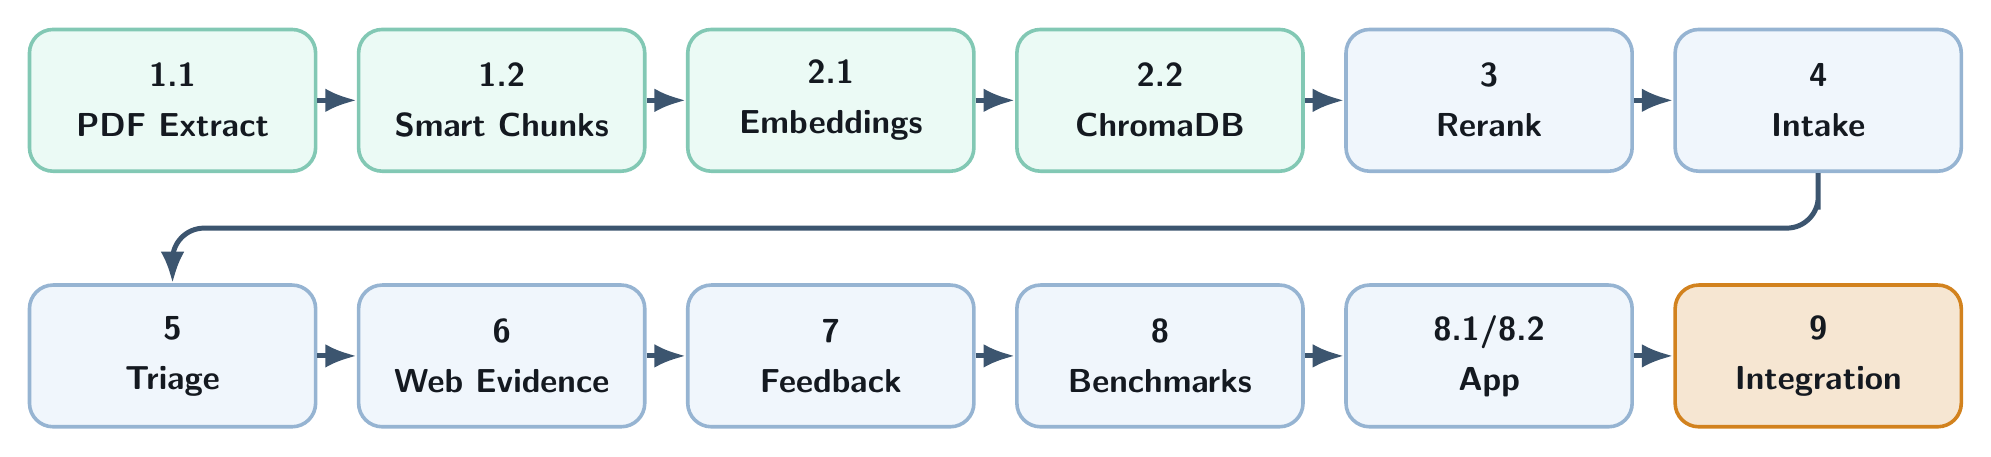
\begin{tikzpicture}[node distance=5mm and 5mm]
  \node[data, text width=34mm] (p1) {1.1\\PDF Extract};
  \node[data, text width=34mm, right=of p1] (p2) {1.2\\Smart Chunks};
  \node[data, text width=34mm, right=of p2] (p3) {2.1\\Embeddings};
  \node[data, text width=34mm, right=of p3] (p4) {2.2\\ChromaDB};
  \node[sys, text width=34mm, right=of p4] (p5) {3\\Rerank};
  \node[sys, text width=34mm, right=of p5] (p6) {4\\Intake};
  \node[sys, text width=34mm, below=14mm of p1] (p7) {5\\Triage};
  \node[sys, text width=34mm, right=of p7] (p8) {6\\Web Evidence};
  \node[sys, text width=34mm, right=of p8] (p9) {7\\Feedback};
  \node[sys, text width=34mm, right=of p9] (p10) {8\\Benchmarks};
  \node[sys, text width=34mm, right=of p10] (p11) {8.1/8.2\\App};
  \node[data, draw=accentamber, fill=accentamber!20, text width=34mm, right=of p11] (p12) {9\\Integration};
  \draw[flow] (p1) -- (p2); \draw[flow] (p2) -- (p3); \draw[flow] (p3) -- (p4); \draw[flow] (p4) -- (p5); \draw[flow] (p5) -- (p6);
  \draw[flow, rounded corners=4mm] (p6) |- ($(p6.south)+(0,-7mm)$) -| (p7.north);
  \draw[flow] (p7) -- (p8); \draw[flow] (p8) -- (p9); \draw[flow] (p9) -- (p10); \draw[flow] (p10) -- (p11); \draw[flow] (p11) -- (p12);
\end{tikzpicture}
\end{center}
\vspace{5mm}
{\SmallFont
\begin{tabular}{p{0.31\linewidth}p{0.60\linewidth}}
\toprule
\textbf{Engineering layer} & \textbf{Concrete implementation evidence}\\
\midrule
Corpus & PyMuPDF parser, per-font PUA correction, two-column ordering\\
Retrieval & medical embeddings, ChromaDB metadata filters, BGE reranking\\
Agents & LangGraph intake, Mode A/Mode B triage, patient memory\\
Application & FastAPI, PostgreSQL, React/TypeScript, doctor-only reports\\
\bottomrule
\end{tabular}}

\vspace{3mm}
{\SmallFont\color{muted}\textbf{Output:} clean sections, chunk JSON, embedding matrix, vector store, RAG traces, diagnosis reports, feedback JSONL, and EC2/Ollama deployment preparation.}
}{navy}

% ---------------------------------------------------------------------------
% Right column
% ---------------------------------------------------------------------------
\panel{810}{410}{350}{175}{Formal Testing \& Benchmark Analysis}{%
\vspace{-4mm}
\begin{center}
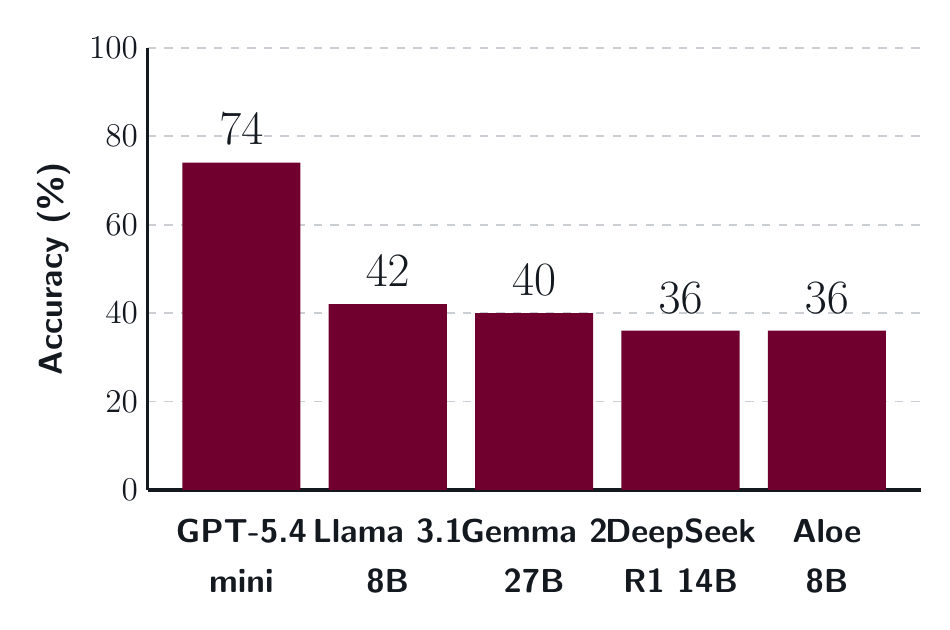
\begin{tikzpicture}
\begin{axis}[
    ybar,
    bar width=15mm,
    width=0.94\linewidth,
    height=72mm,
    ymin=0, ymax=100,
    enlarge x limits=0.16,
    ylabel={\textbf{Accuracy (\%)}},
    ylabel style={font=\TinyFont, text=ink},
    symbolic x coords={GPT,Llama,Gemma,DeepSeek,Aloe},
    xtick=data,
    xticklabels={
        {GPT-5.4\\mini},
        {Llama 3.1\\8B},
        {Gemma 2\\27B},
        {DeepSeek\\R1 14B},
        {Aloe\\8B}
    },
    x tick label style={
        font=\bfseries\TinyFont,
        text=ink,
        align=center,
        yshift=-1mm
    },
    y tick label style={font=\TinyFont, text=ink},
    nodes near coords,
    every node near coord/.append style={
        font=\bfseries\SmallFont,
        text=ink,
        yshift=1mm
    },
    axis line style={line width=1.2pt, draw=ink},
    ymajorgrids=true,
    grid style={line width=0.7pt, dashed, draw=muted!30},
    axis x line*=bottom,
    axis y line*=left,
    tick style={draw=none},
    clip=false
]
\addplot[fill=aub, draw=none] coordinates {
    (GPT,74)
    (Llama,42)
    (Gemma,40)
    (DeepSeek,36)
    (Aloe,36)
};
\end{axis}
\end{tikzpicture}
\end{center}

\vspace{-1mm}
{\SmallFont
\textbf{Conclusion from tests.}
GPT-5.4-mini is the API-model comparison ceiling. The other bars are open-source/local RAG runs for the hospital-deployable path. RAG is strongest when CMDT contains the answer; on rare MedCaseReasoning cases, RAG reached 30\%, while governed web search reached 42\%.
}
}{aub}

\panel{810}{250}{350}{130}{Evaluation Matrix}{%
\vspace{-2mm}
{\SmallFont
\renewcommand{\arraystretch}{1.18}
\begin{tabular}{p{0.27\linewidth}p{0.36\linewidth}p{0.27\linewidth}}
\toprule
\textbf{\color{navy}Layer} & 
\textbf{\color{navy}Formal Test} & 
\textbf{\color{navy}Result}\\
\midrule
Data quality & PUA scan after PDF extraction & 0 remaining\\
Chunking & Structured chunks vs baseline & 5,631 chunks\\
Retrieval & Hit@k, MRR, metadata filters & 100\% Hit@3\\
Reranking & Offline content judge & 4.35/5 BGE\\
Agents & Scenario-based tests & Red flags + follow-ups\\
Web evidence & Privacy, source quality, JSON & 100\% pass\\
Application & Roles, reports, feedback & Doctor-only diagnosis\\
\bottomrule
\end{tabular}
}

\vspace{2mm}
{\SmallFont\color{muted}
\textbf{Why this matters:} Evaluation follows the full pipeline from corpus quality to application behavior, not only the final diagnosis output.
}
}{accentteal}

\panel{810}{100}{350}{120}{Representative Clinical Workflows}{%
{\SmallFont
\begin{tabular}{p{0.23\linewidth}p{0.67\linewidth}}
\toprule
\textbf{Case} & \textbf{Doctor-facing output}\\
\midrule
Mode A: chest pain + hemoptysis & Primary provisional diagnosis: \textbf{Pulmonary Embolism}; differentials: ACS, Aortic Dissection, Pericarditis; tests: CTPA, D-dimer, ECG, troponin, chest X-ray.\\
Mode B: painful leg nodules + fever & Refined uncommon presentation to \textbf{Erythema Nodosum}; suggested workup: ASO/strep, chest X-ray, TB test, ESR/CRP, medication review.\\
Doctor review & Physician confirms, rejects, or corrects the report; feedback becomes future supervised training data.\\
\bottomrule
\end{tabular}}

\vspace{2mm}
{\TinyFont\color{muted}\textit{Representative functional tests, not clinical validation.}}
}{navy}

% ---------------------------------------------------------------------------
% Bottom conclusion band
% ---------------------------------------------------------------------------
\fill[navy] (0,0) rectangle (1189,82);
\node[anchor=west, align=left, text=white] at (35,42) {%
  \begin{minipage}{250mm}
  {\PanelTitleFont Conclusion}\vspace{1mm}\\
  {\TinyFont\color{white!80}Main claim of the poster}
  \end{minipage}
};
\node[anchor=west, align=left, text=white] at (300,42) {%
  \begin{minipage}{840mm}
  \BodyFont\RaggedRight
  Medora demonstrates a complete engineering path from raw CMDT text to structured intake, evidence-grounded provisional triage, privacy-safe current evidence, doctor feedback, and full-stack clinical review. The system preserves the core safety boundary: \textbf{final diagnosis belongs to the clinician.} \textcolor{white!78}{Next: clinician-labeled validation, Arabic/multilingual intake, production security, and persistent distributed agent sessions.}
  \end{minipage}
};

\end{tikzpicture}
\end{document}
